%%%%%%%%%%%%%%%%%%%%%%%%%%%%%%%%%%%%%%%%%%%%%%%%%%%%%%%%%%%%%%%%%%%%%%%%%%%%%%%%%%%%%%%%%%%%%%%%%%%%%%%%%%%%%%%%%%%%%%%%%%%%%%%%%%%%%%%%%%%%%%%%%%%%%%%%%%%
% This is just an example/guide for you to refer to when submitting manuscripts to Frontiers, it is not mandatory to use Frontiers .cls files nor frontiers.tex  %
% This will only generate the Manuscript, the final article will be typeset by Frontiers after acceptance.   
%                                              %
%                                                                                                                                                         %
% When submitting your files, remember to upload this *tex file, the pdf generated with it, the *bib file (if bibliography is not within the *tex) and all the figures.
%%%%%%%%%%%%%%%%%%%%%%%%%%%%%%%%%%%%%%%%%%%%%%%%%%%%%%%%%%%%%%%%%%%%%%%%%%%%%%%%%%%%%%%%%%%%%%%%%%%%%%%%%%%%%%%%%%%%%%%%%%%%%%%%%%%%%%%%%%%%%%%%%%%%%%%%%%%

%%% Version 3.4 Generated 2022/06/14 %%%
%%% You will need to have the following packages installed: datetime, fmtcount, etoolbox, fcprefix, which are normally inlcuded in WinEdt. %%%
%%% In http://www.ctan.org/ you can find the packages and how to install them, if necessary. %%%
%%%  NB logo1.jpg is required in the path in order to correctly compile front page header %%%

\documentclass[utf8]{FrontiersinHarvard} % for articles in journals using the Harvard Referencing Style (Author-Date), for Frontiers Reference Styles by Journal: https://zendesk.frontiersin.org/hc/en-us/articles/360017860337-Frontiers-Reference-Styles-by-Journal
%\documentclass[utf8]{FrontiersinVancouver} % for articles in journals using the Vancouver Reference Style (Numbered), for Frontiers Reference Styles by Journal: https://zendesk.frontiersin.org/hc/en-us/articles/360017860337-Frontiers-Reference-Styles-by-Journal
%\documentclass[utf8]{frontiersinFPHY_FAMS} % Vancouver Reference Style (Numbered) for articles in the journals "Frontiers in Physics" and "Frontiers in Applied Mathematics and Statistics" 

%\setcitestyle{square} % for articles in the journals "Frontiers in Physics" and "Frontiers in Applied Mathematics and Statistics" 
\usepackage{xcolor,url,hyperref,lineno,microtype,subcaption}
\usepackage[onehalfspacing]{setspace}
\usepackage{colortbl} % Required for coloring table cells

\linenumbers


% Leave a blank line between paragraphs instead of using \\


\def\keyFont{\fontsize{8}{11}\helveticabold }
\def\firstAuthorLast{Steinert {et~al.}} %use et al only if is more than 1 author
\def\Authors{Sven J. Steinert\,$^{1,*}$, Paul Zabel\,$^{2}$ and Dominik Quantius\,$^{2}$}
% Affiliations should be keyed to the author's name with superscript numbers and be listed as follows: Laboratory, Institute, Department, Organization, City, State abbreviation (USA, Canada, Australia), and Country (without detailed address information such as city zip codes or street names).
% If one of the authors has a change of address, list the new address below the correspondence details using a superscript symbol and use the same symbol to indicate the author in the author list.
\def\Address{$^{1}$School of Engineering and Design, Technical University of Munich (TUM), Munich, Germany \\
$^{2}$Institute of Space Systems, Systemanalyse Raumsegment, German Aerospace Center (DLR), Bremen, Germany}
% The Corresponding Author should be marked with an asterisk
% Provide the exact contact address (this time including street name and city zip code) and email of the corresponding author
\def\corrAuthor{Sven Julius Steinert}

\def\corrEmail{sven.julius.steinert@outlook.com}


\begin{document}
\onecolumn
\firstpage{1}

\title {Location dependent flight cost differences from the lunar surface to an orbital fuel depot and its influence on ISRU location selection} 

\author[\firstAuthorLast ]{\Authors} %This field will be automatically populated
\address{} %This field will be automatically populated
\correspondance{} %This field will be automatically populated

\extraAuth{}% If there are more than 1 corresponding author, comment this line and uncomment the next one.
%\extraAuth{corresponding Author2 \\ Laboratory X2, Institute X2, Department X2, Organization X2, Street X2, City X2 , State XX2 (only USA, Canada and Australia), Zip Code2, X2 Country X2, email2@uni2.edu}

\maketitle

\begin{abstract}

%%% Leave the Abstract empty if your article does not require one, please see the Summary Table for full details.
\section{}
With increasing relevance for lunar activities, the location selection for ISRU facilities is a necessary step to identify the most suitable configuration during mission planning.
To raise information about the dominant location dependencies, a scenario was set up where an ISRU product is exported to an orbital depot and mass costs are used for classification. 
In the selected scenario, Oxygen is produced by an Ilmenite reduction plant and subsequently exported to the Lunar Gateway via an Oxygen-Hydrogen fueled launcher running in a round-trip, refueling Oxygen at the lunar surface and Hydrogen at the Lunar Gateway.
It showed that the variations in transport costs can be either entirely avoided or have a recessive influence on the mission's total costs over an extended amount of time, such as 20 years.
The identification of the top 10 most optimal locations for various resolutions were only slightly altered under consideration of flight costs compared to only considering the ISRU factors, which concludes the insignificance of flight cost dependencies for the analysed case.

\tiny
 \keyFont{ \section{Keywords:} In situ resource utilization (ISRU), orbital fuel depot, delta v map, lunar outpost, location selection, Ilmenite reduction, Lunar Gateway, Near-rectilinear halo orbit (NRHO)} %All article types: you may provide up to 8 keywords; at least 5 are mandatory.
\end{abstract}

\section{Introduction}

% cite like this: \citep{name}

The Moon and its currently unused resources are holding a great potential in economics and development for the human presence.
The big collaborative field study of \cite{Kornuta2019} has shown, that an undertaking like this is technologically feasible which was presented in a commercial architecture. In contrast to \cite{Kornuta2019}, where water ice in the permanently shadowed regions near the poles is focused as resource for Hydrogen and Oxygen via electrolysis, Oxygen could be also obtained through extraction from regolith.
This involves downsides as Oxygen is only one propellant component and big machinery for regolith handling is required, but also opportunities as the abundance of Oxygen in regolith is truly vast with a combined weight percent up to 45\% measured from Apollo return samples in \cite{Papike1982}.
This Oxygen is bonded to various elements which is where extraction methods as Hydrogen reduction of Ilmenite are focusing on one specific bond for an effective processing procedure.
Therefore propellant production does not need to be restricted to the polar regions, especially when a fully robotic In situ resource utilization (ISRU) plant is feasible on the lunar surface and no life support systems and their water resources are required. 
Optimization can be therefore based on the process factors to pick the most optimal location globally.
For this event, the goal of this analysis is to identify the leading significance of two sections of process factors, the ISRU efficiency and the transport efficiency.
In case of insignificance by one of these influences, a prioritization is provided for future mission analysis on similar scenarios.


\section{Materials and methods}

The determination of influences is approached by an example scenario under which both ISRU hardware costs and flight costs can be assigned and put together into a joined model under which comparisons can be drawn, through mass costs as central unit.
The example scenario consists out of an ISRU Oxygen plant on the lunar surface and an orbital fuel depot where a comparable launcher is delivering and consuming the produced Oxygen.

%The method of ISRU Oxygen production is specified to Ilmenite reduction, where location dependent ISRU hardware mass costs are determined through raw material concentration data of Ilmenite ressources via TiO2 from \cite{Sato.2017} in combination with estimates around Highland and Mare classification from \cite{Nelson.2014} and finally transferred to hardware mass costs by a function of a scalable Ilmenite reduction facility from \cite{GuerreroGonzalez2023}.

\subsection{ISRU Efficiency}
\label{sec:A}
When the optimal location is chosen by the highest ISRU efficiency, the whole production line has to be inspected for location dependent factors first.
Such location dependent factors are for example: raw material concentration, solar irradiance, temperatures, flat surface conditions and further scenic requirements.
Hereby, the production method is decisive about the sensitivity to location depended factors.
One prominent extraction method is the Hydrogen reduction of Ilmenite which has been already demonstrated as in \cite{Sargeant2020}. In this process, the chemical bond of $FeTiO_3$ is broken down by Hydrogen resulting in the chemical Equation \ref{eq:ilmenite-reduction}. The resulting water is electrolyzed where the Hydrogen is fed back and the net reaction leaves pure Oxygen.

\begin{equation}
FeTiO_3 + H_2 \longrightarrow Fe + TiO_2 + H_2O
\label{eq:ilmenite-reduction}
\end{equation}

Hydrogen reduction of Ilmenite is chosen as the production method to be analyzed, which we expect to feature a high dependency on the raw material concentration and therefore a strong location dependency due to inhomogeneity of Ilmenite distribution.
An alternative extraction method would be molten regolith electrolysis which is mostly invariant over the lunar surface, which is why all results that are derived here are therefore only applicable to the chosen production method.

\subsubsection{Model}
\label{sec:model}
To reduce model complexity, our model does include only the raw material concentration factor as argument, the Ilmenite weight ratio $w_{\mathrm{ilmenite}}$.
While this does not cover all influences, the raw material concentration covers a major part for the location dependency and does therefore serve as approximation to a full location dependent model of Hydrogen reduction of Ilmenite.
The hardware mass that has to be moved to the lunar surface for ISRU operation serves as the criteria to be minimized. In a previous work of \citep{GuerreroGonzalez2023} this hardware mass $m_{hardware}$ depending on Ilmenite concentration was determined for a combined production plant of Low Carbon Steel and Oxygen production. This production plant was sized for an annually output of 23.9 t Oxygen and 25 t Low Carbon Steel. The model consists out of a sum of required subsystems as defined in Equation \ref{eq:ISRU_model} \citep{GuerreroGonzalez2023}.

\begin{alignat*}{2}
    & y_{0}(x) =  \ \ 4036 \cdot x^{-1.064} \ -9.59   && \qquad \text{Excavation}                  \\
    & y_{1}(x) =  17580 \cdot x^{-1.003} \  -390.8    && \qquad \text{Handling}                    \\
    & y_{2}(x) =  19240 \cdot x^{-1.003} \  -421.9    && \qquad \text{Beneficiation}               \\
    & y_{3}(x) =  21780 \cdot x^{-1.198} \  +120.3    && \qquad \text{O2 Extraction}               \\
    & y_{4}(x) =  17910 \cdot x^{-1.265} \  +1370     && \qquad \text{O2 Purification}             \\
    & y_{5}(x) =  29650 \cdot x^{-0.7005} -602.5      && \qquad \text{Metal Processing}            \\
    & y_{6}(x) =  \ \ 2541 \cdot x^{-0.7434}  +286.8  && \qquad \text{Gas Liquefaction \& Storage}  \\ 
    & y_{7}(x) =  32440 \cdot x^{-0.8312}  +125.2     && \qquad \text{Thermal Control}             \\
    & y_{8}(x) =  12000 \cdot x^{-0.9657}  +63.99     && \qquad \text{Power}
\end{alignat*}
\begin{equation}
\displaystyle \mathrm{m_{hardware}}(x=w_{\mathrm{ilmenite}} \ [wt\%]) = \sum\limits_{i=0}^8 y_{i}(x) \ [kg]
\label{eq:ISRU_model}
\end{equation}

 Where in our scenario, only the Oxygen production is relevant, the additional subsystems as metal processing scale in a similar way as the rest of the system so that the spread between low and high values of $w_{\mathrm{ilmenite}}$ is not distorted significantly (88.69\%  spread to the maximum value vs. 89.97\% spread without metal processing, for $1 \ wt\% \leq w_{\mathrm{ilmenite}} \leq 11 \ wt\%$). Furthermore, this combined production plant could still be a viable choice out of the synergistic effects of shared infrastructure. This is why we are choosing this model to be our reference production plant as a whole rather than trimming subsystems. Therefore our model is expressed in Equation \ref{eq:ISRU_model} as well.

\subsubsection{Data Processing}
To determine the cost for every location on the Moon, a global lunar map of Ilmenite weight ratio is required. In a previous work by Hiroyuki Sato \citep{Sato.2017} an almost global TiO2 abundance map was created, where the values of weight percent (wt\%) for TiO2 are used as equivalent for Ilmenite. The resulting map had a mask applied to leave only lunar Mare regions and had a limited latitude coverage from $-70^{\circ}$ to $70^{\circ}$. The limited coverage originates from the orbiter sensor data and its limitations in measurement at an increasingly steep sunlight angle towards the poles. The initial data was created by the Lunar Reconnaissance Orbiter Camera (LROC) Wide Angle Camera (WAC) which is our starting point to recreate a similar dataset as \citep{Sato.2017} but on a global basis.
The original WAC data segments are joined together in Figure \ref{fig:TiO2-original}.

\begin{figure}[h!]
\begin{center}
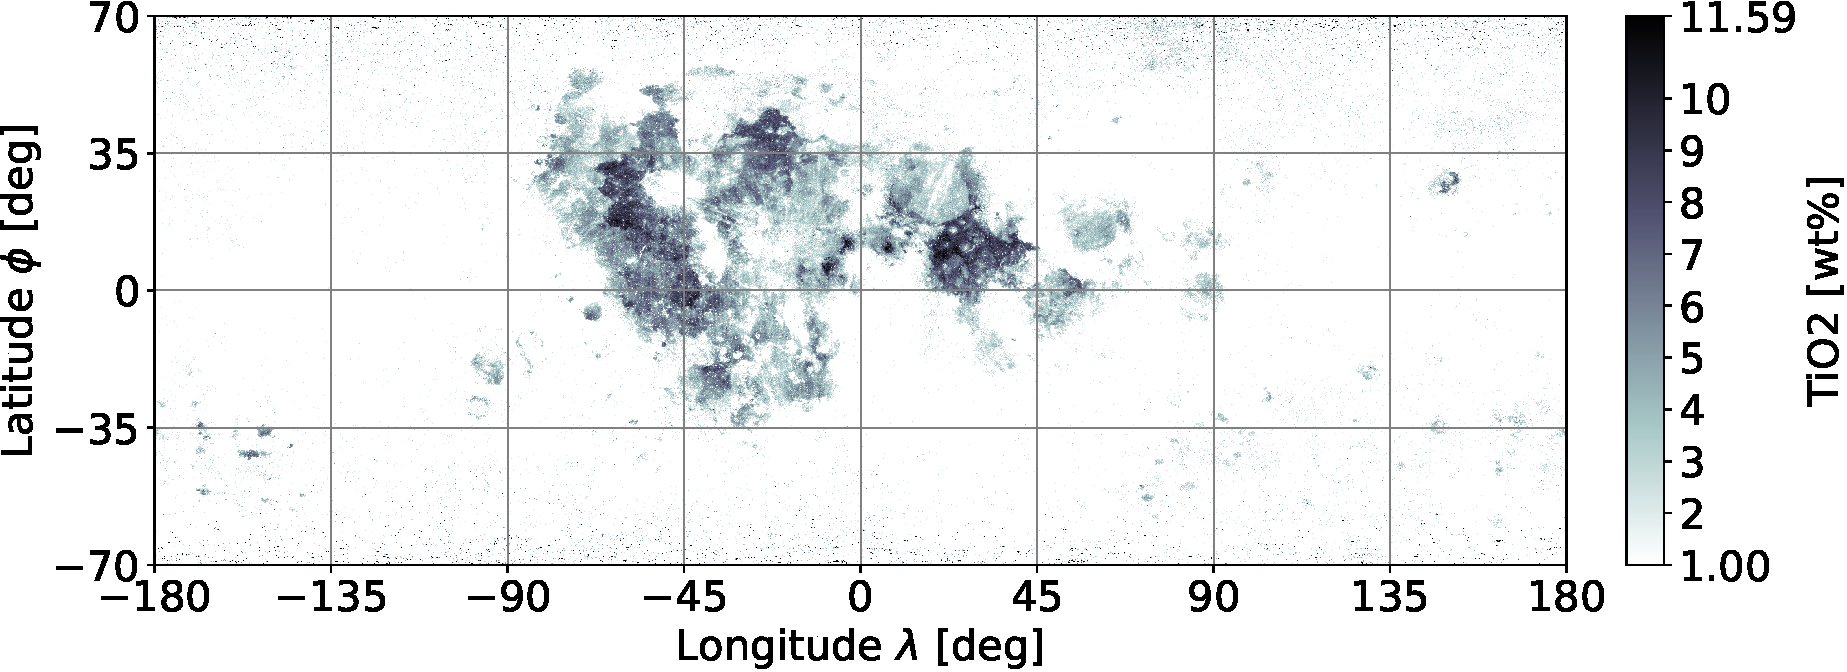
\includegraphics[width=\linewidth]{img/WAC_TIO2_COMBINED.pdf}
\end{center}
\caption{Combined original TiO2 data of the WAC, \citep{Sato.2017}}
\label{fig:TiO2-original}
\end{figure}

\newpage
\paragraph{Cleanup and Estimation}
One problem are unusual high measurements towards the poles that are considered increasing noise which is scattered through the entire longitudinal axis.
The second problem is the incomplete coverage of latitude and therefore the poles itself.
To derive an estimation over the missing information at latitudinal coverage, the following strategy is applied.
If Ilmenite abundance correlates with the classification of Highlands / Mare and the pole regions geology is featuring highland characteristics then the expected value of the known highland region serves as an estimate of Ilmenite content at the poles.


\begin{figure}[h!]
\begin{center}
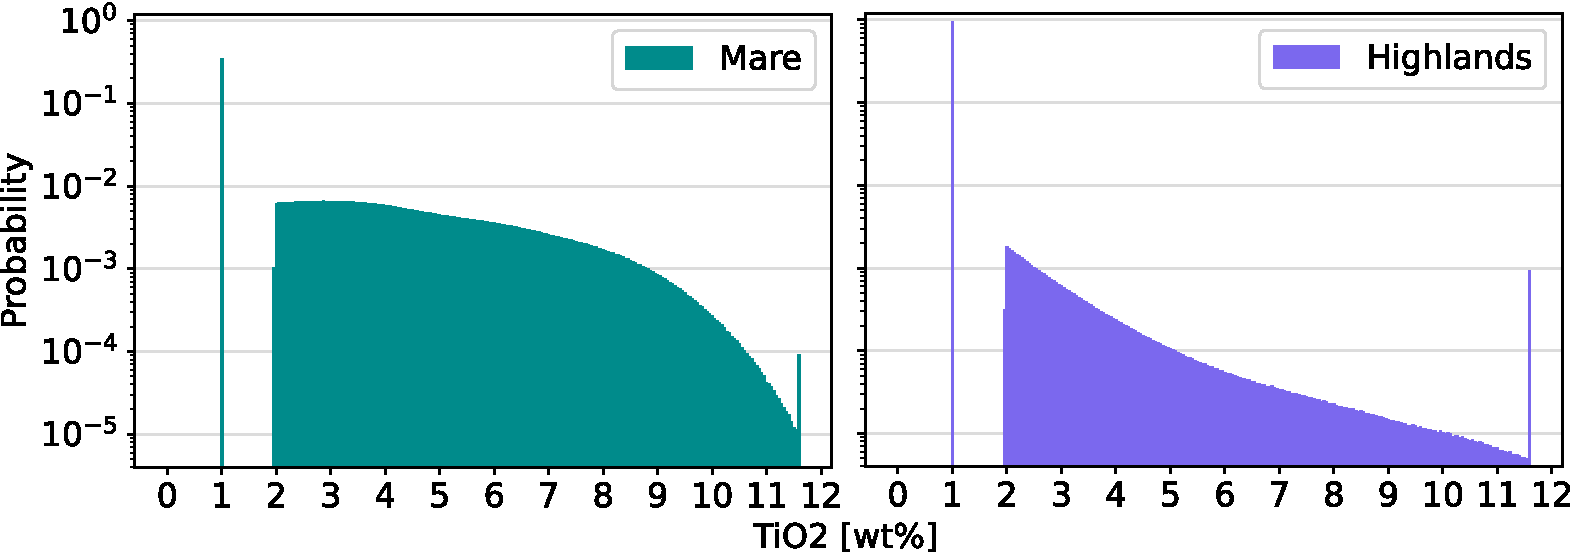
\includegraphics[width=\linewidth]{img/WAC_TIO2_CLUSTERING.pdf}
\end{center}
\caption{Distribution of Ilmenite content clustered into Highlands and Mare (equirectangular corrected) on combined WAC data with Mare boundaries from \citep{Nelson.2014}}
\label{fig:TiO2-Highlands-Mare-Distribution}
\end{figure}


As Figure \ref{fig:TiO2-Highlands-Mare-Distribution} shows, the distribution characteristics of these two regions deviate considerably, whereby the average abundance also differs from 3,38 wt\% in Mare to 1,1 wt\% in Highland regions. Therefore the Ilmenite content correlation is given and the estimate over the missing latitudinal area of Highlands is set to 1 wt\% which also matches the WAC original assumption for values under the detection ratio.
To additionally remove the increasing noise at further extreme latitudes, a mask is created out of  Mare boundaries from \citep{Nelson.2014} merged with a constant separation at $\phi = \pm56 ^{\circ}$. The replacement values for the mask are equally set to 1 wt\%.
With both estimates applied, a low noise global Ilmenite map is accomplished which can be seen in Figure \ref{fig:Ilmenite-map}.

\begin{figure}[h!]
\begin{center}
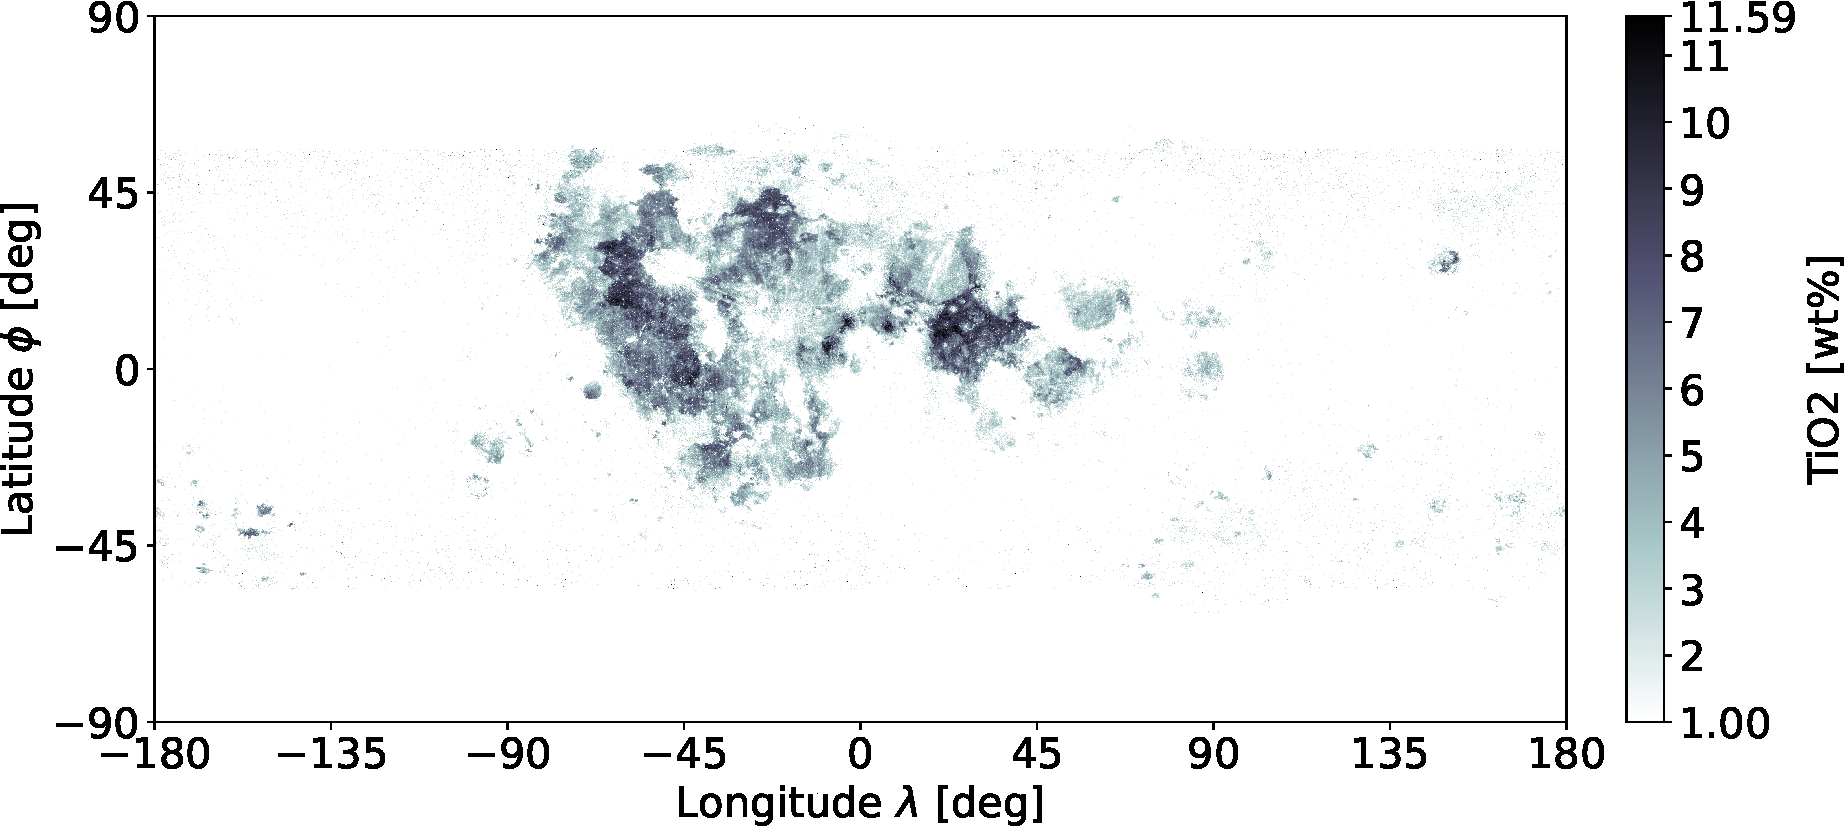
\includegraphics[width=\linewidth]{img/WAC_TIO2_GLOBAL.pdf}
\end{center}
\caption{Global lunar Ilmenite map in weight percent through TiO2, based on WAC data and estimates}
\label{fig:Ilmenite-map}
\end{figure}


\paragraph{ISRU Mass Cost Map}

This global Ilmenite abundance map from Figure \ref{fig:Ilmenite-map} is now used as input to  Equation \ref{eq:ISRU_model}, which is resulting in the location dependent ISRU hardware mass displayed in Figure \ref{fig:A-cost-map}.

\label{sec:ISRU-map}


\begin{figure}[h!]
\begin{center}
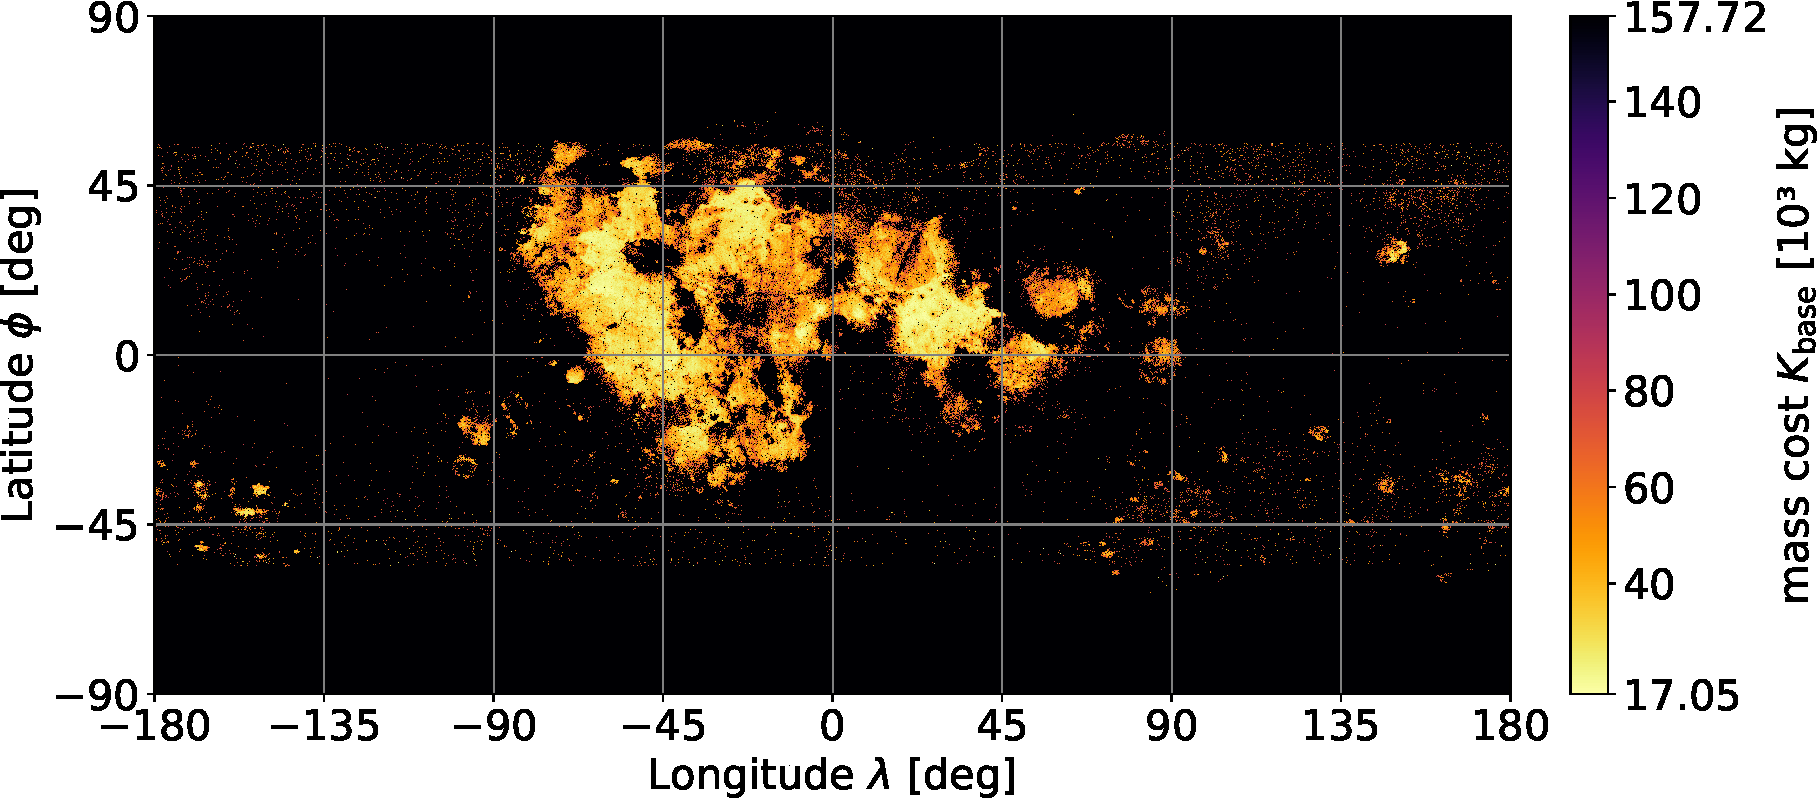
\includegraphics[width=\linewidth]{img/ISRU_COST_GLOBAL.pdf}
\end{center}
\caption{Location dependent ISRU hardware mass cost $K_{\mathrm{base}}$ in its base configuration of 23.9 t Oxygen per year}
\label{fig:A-cost-map}
\end{figure}


\subsection{Transport efficiency}
\label{sec:B}

\subsubsection{Mission Planning}
\label{sec:mission-planning}

The mission is designed to be carried out by a single stage launcher to loop between the lunar surface and the target orbit destination.
The Oxygen fuel component and the Oxygen payload are refilled on lunar ground at the ISRU production plant.
The Hydrogen fuel component on the other hand is refilled at the fuel depot where also the Oxygen payload is delivered.
This results effectively in an exchange of delivered Oxygen to deducted Hydrogen from the station.  
A multi staged launcher or a shuttle exchange system was neglected for this analysis but would hold the potential to further increase the transport efficiency.

\subsubsection{Orbital Fuel Depot Location}
\label{sec:fuel-depot}

The primary requirement of the fuel depot location is its accessibility from both the supplying and consuming units.
For an interplanetary or cis-lunar logistic hub near Earth, Liberation points are especially suited as considered by previous studies from \cite{Perrin2016}.
Similar to Liberation points, their corresponding halo orbits are offering the benefits of accessibility as well.
In the case for an interplanetary logistic hub near Earth which is supplied by the lunar surface, the currently planned Lunar Gateway on its Near-rectilinear halo orbit (NRHO) fits prodigiously as a theoretical test bed for this purpose.
Aditionally, a NRHO fuel depot was also considered in the commercial lunar propellant export study by \cite{Kornuta2019}.
Which is why the Lunar Gateway orbit is chosen to be analysed in this scenario as the export destination and considered a fuel depot.

\subsubsection{Target Orbit}

For the selected fuel depot location at the Lunar Gateway, the target orbit is a specific NRHO that is in a 9:2 Lunar Synodic Resonance with an average perilune of $h_{peri}= 3557 \ km$ and an average orbital period of $T= 6.562 \ days$ \citep{2019NationalAA}. It is worth mentioning that this orbit has a varying polar crossing as well as other time dependent changes in its trajectory which are often simplified to more static conditions for analysis \citep{Whitley.2018}.

\subsubsection{Delta-v Estimation}
\label{sec:dv-est}
First of all, regardless of the mission or the trajectory, planetary conditions such as ground elevation and surface velocity are influencing the required $\Delta v$.
These influences are now briefly assessed for the Moon to determine their relevance.

\paragraph{Celestial Influences}
\label{chap:planetary_influences}
% surface point $(Lat=\phi,Lon=\lambda)$

The initial radial distance to the Moon's center of mass $r(\phi, \lambda)$ influences the ideal $\Delta v$ demand directly as shown for an ascent into a circular orbit at $r_{orbit}$ in Equation \ref{eq:elevation}.

\begin{equation}
\displaystyle \Delta v_{ideal}(\phi,\lambda) = \sqrt{v_{orbit}^2 + v_{ascent}^2} = \sqrt{ \left ( \frac{\mu}{r_{orbit}} \right ) +   \left ( 2 \cdot g_0 \cdot \left [ r(\phi, \lambda) - \frac{r(\phi, \lambda)^2}{r_{orbit}} \right ] \right )  }
\label{eq:elevation}
\end{equation}

Global ground elevation data is now used in the form of a displacement map \citep{nasaSVSMoon}, which originates on Lunar Orbiter Laser Altimeter (LOLA) measurements \citep{LRO.2015}.
The elevation ranges from -9.115 km to 10.757 km with regard to the reference radius $r_{\mathrm{ref}}$ of 1737.4 km and therefore defines $r(\phi,\lambda)$ globally.
The displacement map is shown in Figure \ref{fig:heightmap}.

\begin{figure}[h!]
\begin{center}
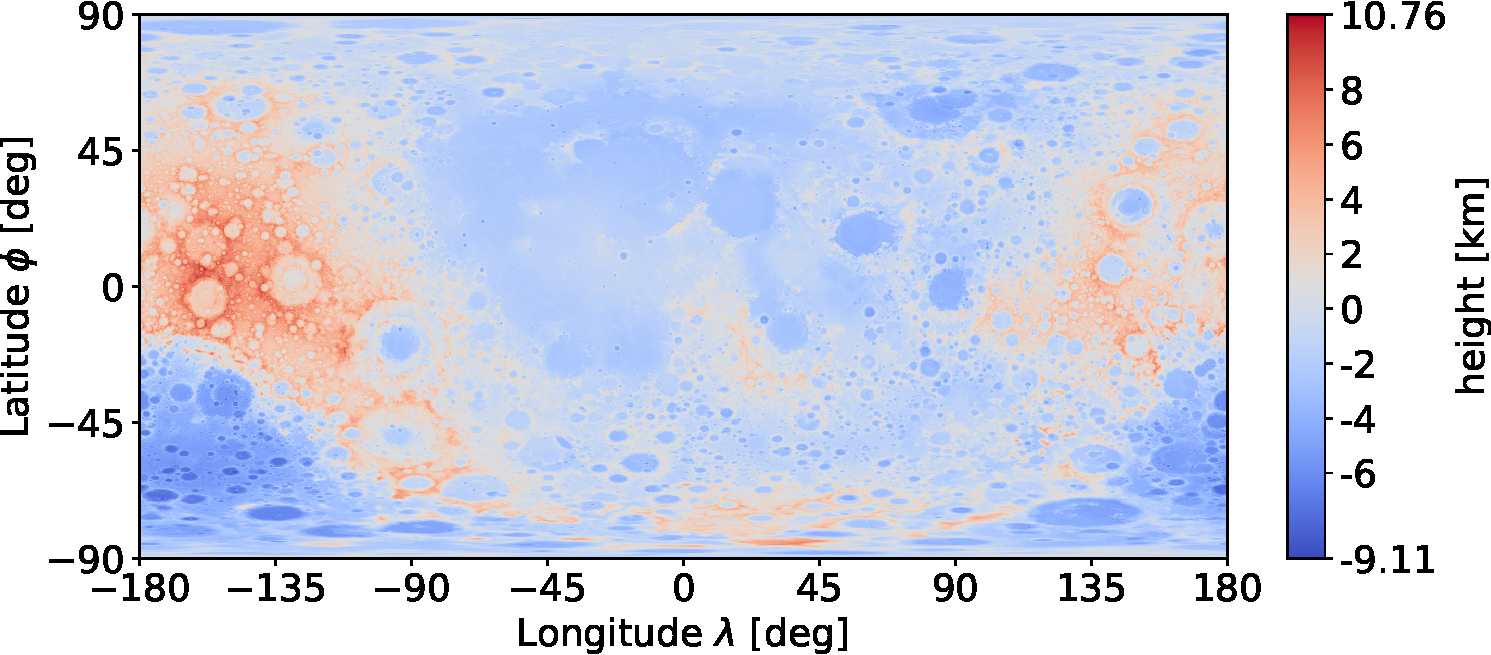
\includegraphics[width=\linewidth]{img/heightmap.pdf}
\end{center}
\caption{Lunar displacement map to reference radius ($r_{\mathrm{ref}}=1737.4 \ km$). Data from NASA CGI Kit \citep{nasaSVSMoon} based on \citep{LRO.2015}}
\label{fig:heightmap}
\end{figure}

Evaluating the extreme values on a Low Lunar Orbit (LLO) at 100 km altitude ($r_{orbit}=1837.4 \ km$) with Equation \ref{eq:elevation} yields:
\begin{equation*}
\begin{array}{ll}
     &  \Delta v_{min}=\Delta v_{ideal}(\max \left \{  r(\phi,\lambda) \right \}= 1725.187 \ \frac{m}{s}\\
     &  \Delta v_{max}=\Delta v_{ideal}(\min \left \{  r(\phi,\lambda) \right \}= 1725.204 \ \frac{m}{s}
\end{array}
\label{eq:heightmap_dv}
\end{equation*}

The influence on $\Delta v$ from ground elevation is therefore at the order of 0.001 \% which is extremely low.

The second celestial influence, the initial surface velocity $v_{0}$ is either an additional $\Delta v$ demand or a $\Delta v$ reduction, depending on the shared velocity components to the launch direction.
Together with the sidereal rotation period and the assumption of a spherical lunar surface of $r_{ref}$, the surface velocity can be given as a function of Latitude $\phi$ as displayed in Equation \ref{eq:groundspeed}.

\begin{equation}
\displaystyle v_{0}(\phi) = \frac{2\pi}{27.322 \ \mathrm{days}} \cdot \cos (\phi) \cdot  r_{\mathrm{ref}}
\label{eq:groundspeed}
\end{equation}

Evaluating the extreme points of polar and equatorial locations on Equation \ref{eq:groundspeed} yields:

\begin{equation*}
\begin{array}{ll}
     &  \Delta v_{min}=\Delta v_{0}(\phi= \pm 90^{\circ}) = 0.000 \ \frac{m}{s}\\
     &  \Delta v_{max}=\Delta v_{0}(\phi=0^{\circ}) = \pm 4.624 \ \frac{m}{s}
\end{array}
\label{eq:groundspeed_dv}
\end{equation*}

Comparing this range $|\Delta v_{max}| - \Delta v_{min}$ to the ascent from the reference radius to a circular 100 km LLO being $\Delta v_{ideal}(r_{ref})=1725.196 \ \frac{m}{s}$ gives the $\Delta v$ influence of the surface velocity to be at the order of 0.27 \% which is significantly more than the elevation influences but still considerably low.

\paragraph{Transfer Options}
\label{sec:transfer-options}

Explicit Transfers from any lunar geodetic point to NRHOs and vice versa are a high-fidelity problem which is usually solved non-analytically as in \citep{Trofimov2020}. Additionally, there are multiple transfer strategies that can be deployed for different optimisation goals. Between optimisation of required $\Delta v$ and transfer time, two transfer options are being analysed for our chosen scenario.

First, a long duration transfer that features a very low required $\Delta v$ of only 664.9 $\frac{m}{s}$ to a LLO at 100 km altitude, which is very close to the theoretical limit of 654.8 $\frac{m}{s}$ as minimum energy change \citep{Whitley.2018}. Also, it features an almost complete independency to surface location, which is reached by something similar to a Three-Impulse transfer, where the lunar sphere of influence is left to circle once around Earth before inserting again. This allows any inclination restrictions to vanish, but at a cost of a 100.1 day long transfer time. If this transfer option is chosen, the influence of transfer efficiency is extremely low and marginal to the ISRU dependencies derived in Chapter \ref{sec:A}. In this case transfer dependencies can be neglected and the location selection can be simplified to only ISRU efficiency.


Often however a 100 day transfer time is simply to long for certain applications, as it for example induces general system lag time and therefore poor dynamics in propellant delivery adjustments in the case of the subjected mission. For this reason, a second transfer option is analysed which is a direct transfer trajectory between the NRHO and the surface from \cite{Trofimov2020}, which features the shortest transfer time of only hours but at the cost of higher $\Delta v$ and location dependency. The direct transfer, illustrated in Figure \ref{fig:NRHO_trajectory}, is the subject of the following analysis in the following sub-chapters.

\begin{figure}[h!]
\begin{center}
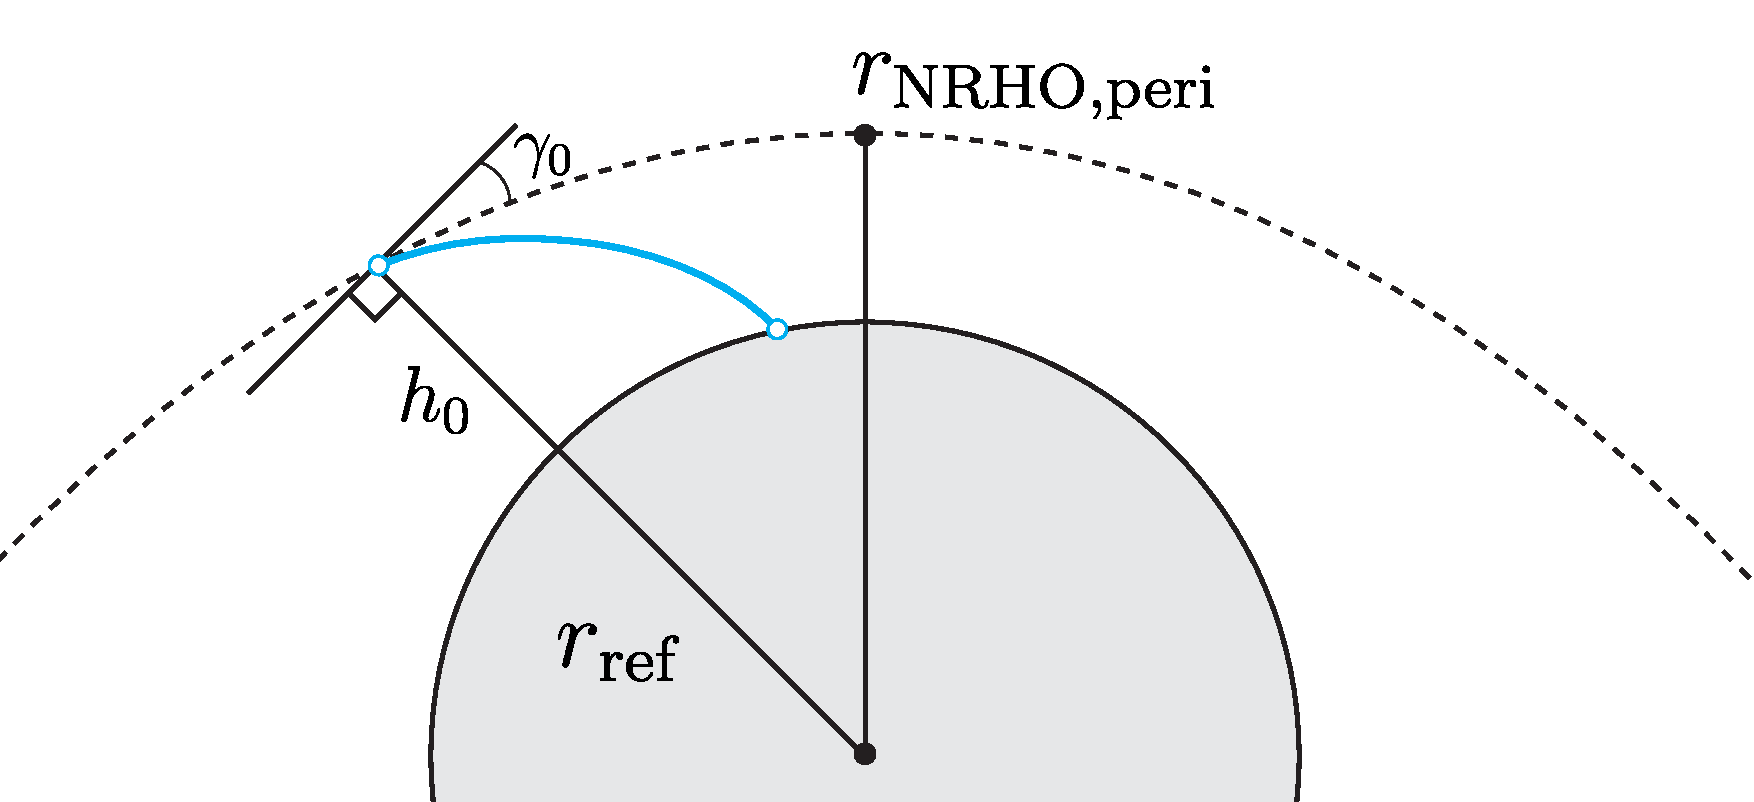
\includegraphics[width=0.6\linewidth]{img/trajectory.pdf}
\end{center}
\caption{Direct ascent trajectory scheme via gravity turn, according to \cite{Trofimov2020}}
\label{fig:NRHO_trajectory}
\end{figure}

\paragraph{Data Processing}
In the previous work by \cite{Trofimov2020}, a set of possible direct decent trajectories and their associated landing point and $\Delta v$ demand were identified. The resulting map of scatter points for the southern 9:2 NRHO was taken as starting point to derive a global $\Delta v$ map.
Since always the cheapest option for one location would be chosen, a minimum estimation was performed.
This estimation was done by splitting the map into $20 \ \mathrm{deg}$ square tiles where constancy is assumed and the lowest value is set for the whole tile.
In preparation for this, the data has been cut from particular high costs trajectories of $\Delta v > 2985.65 \ \frac{m}{s}$ due to rather leaving non defined tiles at the poles than carrying up to $3300 \ \frac{m}{s}$ transfer options over into the final map.
This process is visualized in Figure \ref{fig:dv_processing}.

\begin{figure}[h!]
\begin{center}
\includegraphics[width=\linewidth]{img/dv_processing.pdf}
\end{center}
\caption{Processing of results from \cite{Trofimov2020} (left) to cutting of data (center) into minimum of 20 deg square tiles (right)}
\label{fig:dv_processing}
\end{figure}

The non defined tiles have been linear interpolated along the longitudinal axis, which was only necessary in polar regions where there is already a higher geodetic resolution due to equirectangular projection.
This leads to our final $\Delta v$ map, depicted in Figure \ref{fig:dv_NRHO}. 

\paragraph{Delta v Map}
\label{sec:dv-map}

\begin{figure}[h!]
\begin{center}
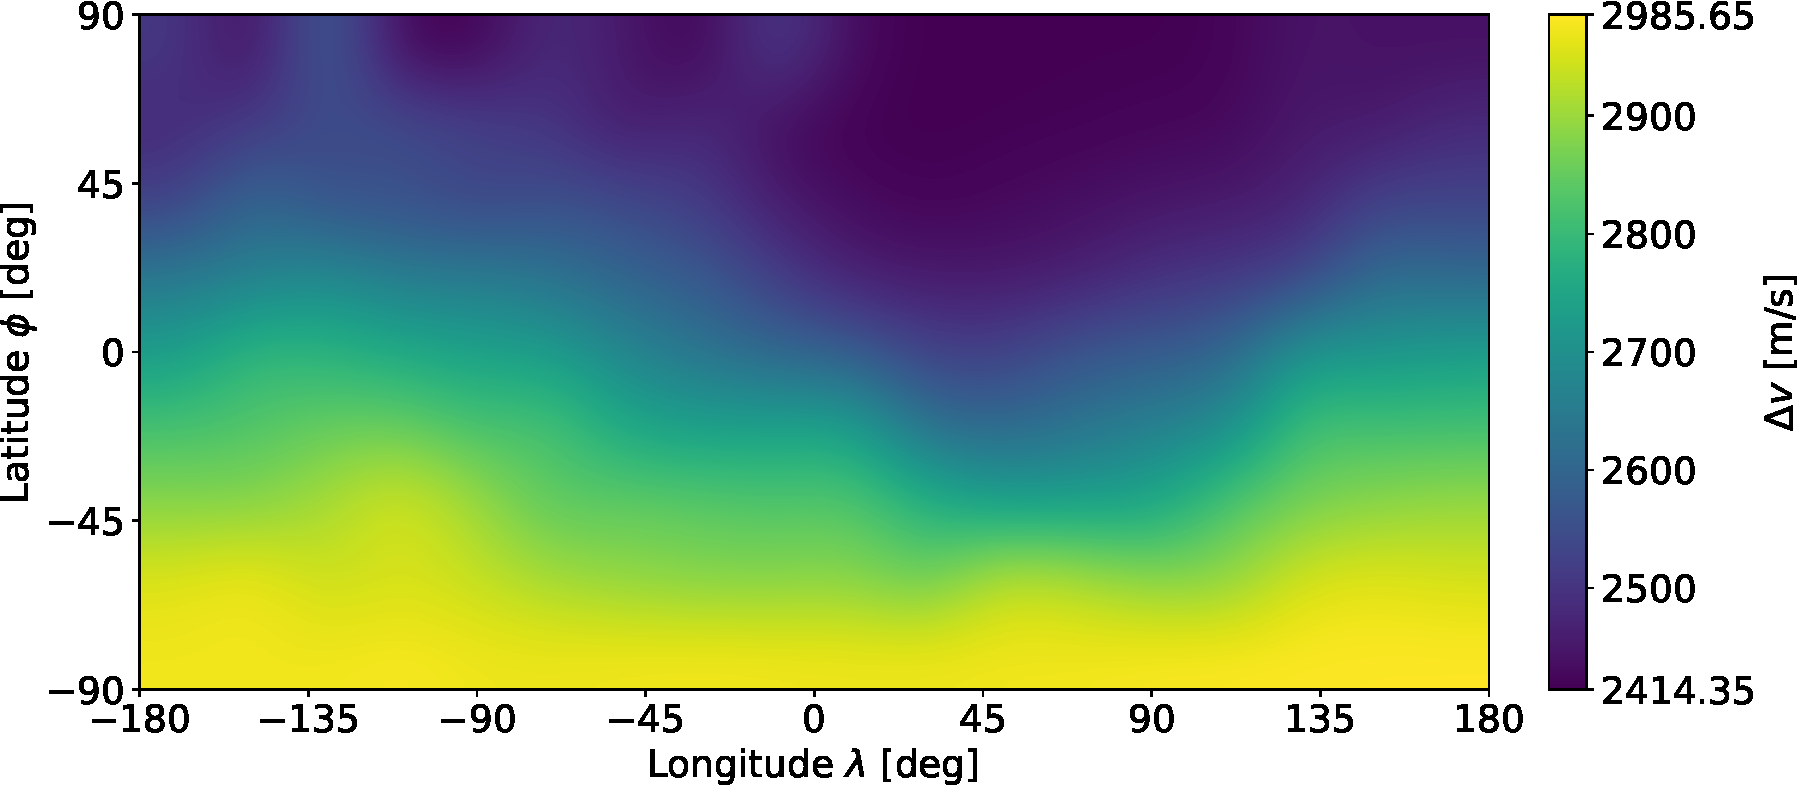
\includegraphics[width=\linewidth]{img/dv_NRHO.pdf}
\end{center}
\caption{Required $\Delta v$ for direct decent from southern 9:2 NRHO to the lunar surface (bicubic interpolated)}
\label{fig:dv_NRHO}
\end{figure}

Even though this data was computed for the decent only, it will serve as estimation for the ascent as well, which is holding a bias as those problems are not entirely symmetric.
Additionally, it should be mentioned that even though a $2414 \ \frac{m}{s}$ transfer is very viable, a transfer of around $2900 \ \frac{m}{s}$ might be rather replaced in a real world scenario by a different transfer strategy, as via a LLO with waiting time to save $\Delta v$.
However in this analysis, Figure \ref{fig:dv_NRHO} defines $\Delta v(\phi,\lambda)$ globally with $\Delta v_{min}=2414.35 \ \frac{m}{s}$ and $\Delta v_{max}=2985.65 \ \frac{m}{s}$.
 

\subsubsection{Transport Carrier}
\label{sec:carrier}
\paragraph{Reference Launcher}
To derive associated transport mass costs, the previously determined $\Delta v$ has to be applied on a specific launcher.
The Argonaut, formerly known as the European Large Logistics Lander (EL3), is chosen as a starting point for this scenario.
The initial configuration is based on the time of writing published information from the \cite{ESA_2023} of 10 000 kg wet mass, 1600 kg dry mass and 2100 kg payload.
Additionally a Hydrogen (H2), Oxygen (O2) propulsion system with an oxidizer fuel ratio of 6 and 400 s of specific impulse are assumed.
When this original configuration is applied on our mission with $\Delta v_{max}$ the fuel is running out before the round-trip can be completed.
Therefore the launcher configuration has to be altered for our scenario needs.

\paragraph{Launcher Up-scaling}
An up-scaling is performed, where the dry mass is kept constant at 1600 kg but fuel is added until the mission can be completed.
The minimal viable system features an empty H2 tank at arrival at the Gateway and an empty O2 tank at the lunar surface.
The Iteration scheme of the up-scaling is visualized in Figure \ref{fig:upscale_iteration} which can now converge a minimal viable launcher for any given payload.
Hereby describes "H2 insufficient" the failure case when the launcher returned but does not have enough H2 to do the next run.

\begin{figure}[h!]
\begin{center}
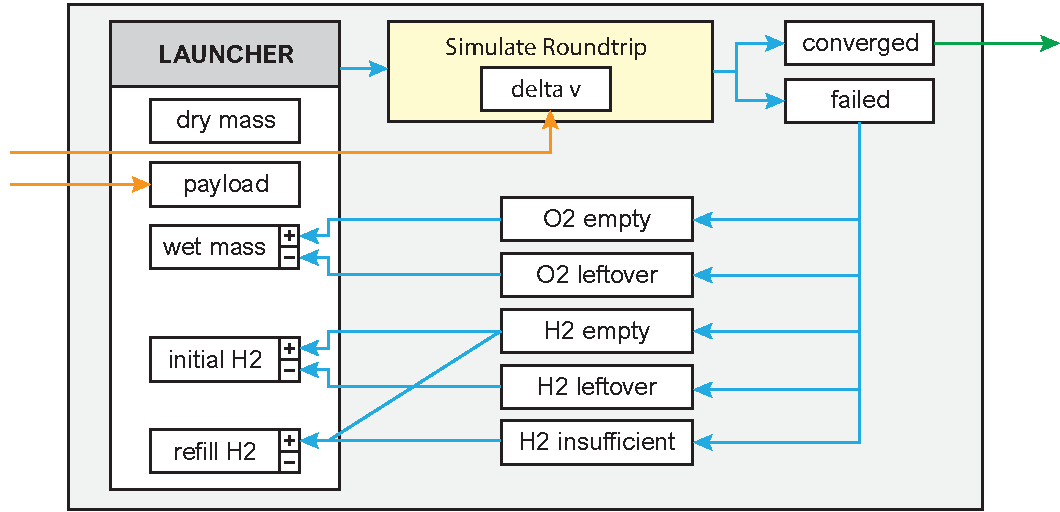
\includegraphics[width=\linewidth]{img/launcher_iteration.pdf}
\end{center}
\caption{Launcher iteration scheme to converge a roundtrip for a given payload and $\Delta v$}
\label{fig:upscale_iteration}
\end{figure}

Since this method of up-scaling is effectively increasing the mass ratio ($r_m = \frac{m_{\mathrm{wet}}}{m_{\mathrm{dry}}}$) of the launcher, this assumption becomes increasingly unrealistic.
Additionally, from the perspective of the fuel depot, Oxygen is delivered but also Hydrogen is taken away, therefore effectively trading those masses by the exchange ratio ($r_{ex} = \frac{m_{\mathrm{payload}}}{m_{\mathrm{H2,refill}}}$).
In order to bring a decision to what range of launchers shall be compared to derive cost differences, Figure \ref{fig:upscale_ratios} visualises the parameter space between the exchange ratio $r_{ex}$ and the mass ratio of the launcher $r_{m}$.

\begin{figure}[h!]
\begin{center}
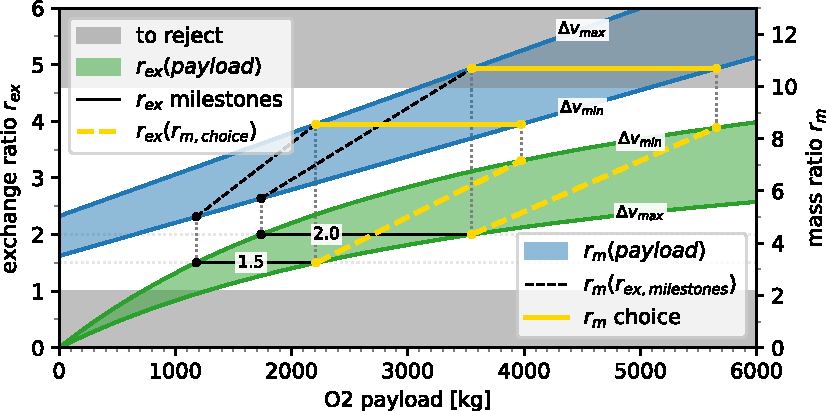
\includegraphics[width=\linewidth]{img/upscale_ratios.pdf}
\end{center}
\caption{Exchange ratio $r_{\mathrm{ex}}$ and mass ratio $r_{\mathrm{m}}$ depending on payload size of the launcher over $\Delta v$ range}
\label{fig:upscale_ratios}
\end{figure}

Hereby there are two sections grayed out, once $r_{ex}<1$ out of economic reasonableness and second $r_{m}>10$ as a soft border of mass ratios for realistic single stage launchers.
The selection of the chosen launcher frames was done through a sequence of movements in the parameter space.
Starting by the economical reasonable exchange ratios of 1.5 and 2.0 (solid black lines, also called milestones), which is then projected to their required mass ratio (dashed black line). This currently holds a set of constant exchange ratio throughout the $\Delta v$ range, in order to obtain comparable results however, the mass ratio $r_m$ has to be constant over one set as it represents the efficiency of the launcher.
Therefore, the maximum value of the mass ratio (at $\Delta v_{max}$) is set as constant over the $\Delta v$ range which is then yielding the chosen frame regarding the mass ratio (solid yellow line).
When this set is then projected back onto the exchange ratio (yellow dashed line), a span of exchange ratios is featured over the $\Delta v$ range.

This concludes the two chosen frames (yellow lines) of:

\begin{equation*}
\begin{array}{ll}
     &  r_{m}=8.555 \quad \mathrm{with} \ \ 1.5 \leq r_{ex} \leq 3.303\\
     &  r_{m}=10.688  \ \ \mathrm{with} \ \ 2.0 \leq r_{ex} \leq 3.889
\end{array}
\label{eq:r_m_choice}
\end{equation*}

To analyse the problem on two frames of different mass ratios is providing insight on the sensitivity towards more efficient launchers in general and their influence on the location selection.





\newpage

\paragraph{Spent Fuel}
\label{sec:spent-fuel}

Through another iteration scheme, which is targeting the chosen mass ratio $r_{\mathrm{m}}$, a launcher can be converged for any $\Delta v$.
The expended fuel is directly drawn from the simulated round-trip and normalized by the payload size, which therefore can be combined into a direct mapping from required $\Delta v$ to the spent fuel $k_{\mathrm{Flight}}$ in kg per kg payload.
This dependency can be seen in Figure \ref{fig:fuel_cost_mapping} for both chosen mass ratios $r_{\mathrm{m}}=8.6$ and $r_{\mathrm{m}}=10.7$.
In this comparison, the higher mass ratio $r_{\mathrm{m}}=10.7$ features a smaller absolute and relative growth, which concludes that differences in spent fuel decrease in general by an increasing launcher efficiency.

\begin{figure}[h!]
\begin{center}
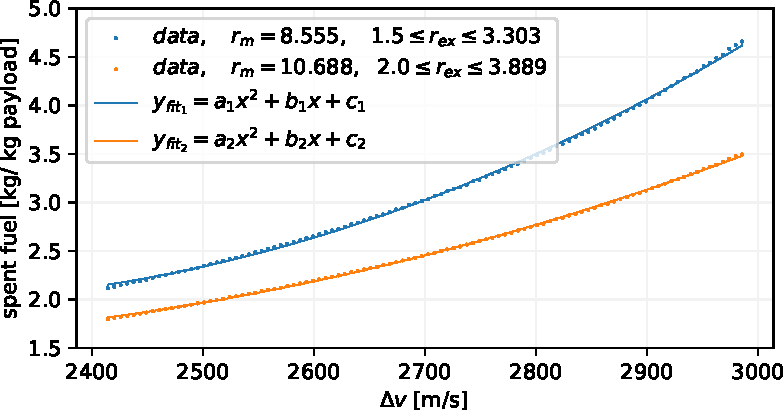
\includegraphics[width=\linewidth]{img/spent_total_mapping.pdf}
\end{center}
\caption{Relationship between required $\Delta v$ and spent fuel $k_{\mathrm{Flight}}$ for both mass ratios}
\label{fig:fuel_cost_mapping}
\end{figure}


\newpage

\subsection{Joined Model}
\label{sec:joined-model}

\subsubsection{Total Cost Modelling}

When both influences from Section \ref{sec:A} and Section \ref{sec:B} are combined, the comparable mass costs have to be drawn from the mission scenario.
Rather than assuming all expended fuel as transport cost, a separation of the fuel components is done, due to the reason that the Oxygen is not being shipped from Earth but rather fully supplied by the ISRU facility.

\paragraph{Fix Costs}
In order to meet the additional demand of Oxygen per year, that the launcher requires for transport, the ISRU facility is scaled up linearly by its ISRU costs per kg Oxygen $k_{\mathrm{ISRU}}$ for each location and its corresponding fuel requirements. 
The scaling factor originates from the base configuration costs from Figure \ref{fig:A-cost-map} and its annual base production $m_{\mathrm{base}}=23.9 \ t$, which gives: $k_{\mathrm{ISRU}}(\phi,\lambda) = \frac{K_{\mathrm{base}}(\phi,\lambda)}{m_{\mathrm{base}}}$.
The additional Oxygen demand per year is derived by the yearly payload $ m_{\mathrm{pl,y}}= 8 \ t$, which has been set to minimize scaling on the base configuration, the oxidiser-fuel-ratio $r_{\mathrm{of}}$ and the spent fuel $k_{\mathrm{Flight}}$ depending on the two selected mass ratios $r_{\mathrm{m}} \in \lbrace 8.6,10.7 \rbrace$.
Therefore the fix costs, which represent the Earth supplied mass for the  construction of the ISRU facility are:

\begin{equation}
\displaystyle K_{\mathrm{Fix}}(\phi,\lambda,r_{\mathrm{m}})=  K_{\mathrm{base}}(\phi,\lambda) +  k_{\mathrm{ISRU}}(\phi,\lambda) \left (  \left [ m_{\mathrm{pl,y}} \cdot k_{\mathrm{Flight}}(\phi,\lambda,r_{\mathrm{m}}) \  \cdot \frac{r_{\mathrm{of}}}{r_{\mathrm{of}}+1} \right ] +  m_{\mathrm{year}} -  m_{\mathrm{base}} \right )
\label{eq:K_fix}
\end{equation}

\paragraph{Dynamic Costs}
The expended Hydrogen is considered fully as mass cost since it is taken from the Lunar Gateway depot and assumed to be delivered by Earth.
Hereby the cost level of the Lunar Gateway and the lunar surface are simplified as equal from Earth to be comparable, which rather overestimates the Hydrogen's cost in comparison to costs on the lunar surface when supplied from Earth.
Therefore the dynamic costs, which represent the Earth supplied mass for Hydrogen on the Lunar Gateway per year $t$ are:

\begin{equation}
\displaystyle K_{\mathrm{Dynamic}}(\phi,\lambda,t,r_{\mathrm{m}}) = t \cdot m_{\mathrm{pl,y}} \cdot  k_{\mathrm{Flight}}(\phi,\lambda,r_{\mathrm{m}}) \  \cdot \frac{1}{r_{\mathrm{of}}+1}
\label{eq:K_dyn}
\end{equation}

\paragraph{Total Costs}
Combining both $K_{\mathrm{Fix}}$ and $K_{\mathrm{Dynamic}}$, the final total costs of the mission over location and time are:

\begin{equation}
\displaystyle K_{\mathrm{Total}}(\phi,\lambda,t,r_{\mathrm{m}}) = K_{\mathrm{Fix}}(\phi,\lambda,r_{\mathrm{m}}) + K_{\mathrm{Dynamic}}(\phi,\lambda,t,r_{\mathrm{m}})
\label{eq:K_total}
\end{equation}


\label{sec:total-map}

Applying Equation \ref{eq:K_total} with location dependent results from Section \ref{sec:ISRU-map} and Section \ref{sec:spent-fuel} gives the total cost maps for the mission time of 20 years for $r_{\mathrm{m}}=8.6$ in Figure \ref{fig:Total_Cost_NRHO_1_5} and $r_{\mathrm{m}}=10.7$ in Figure \ref{fig:Total_Cost_NRHO_2_0}.

\begin{figure}[h!]
\begin{center}
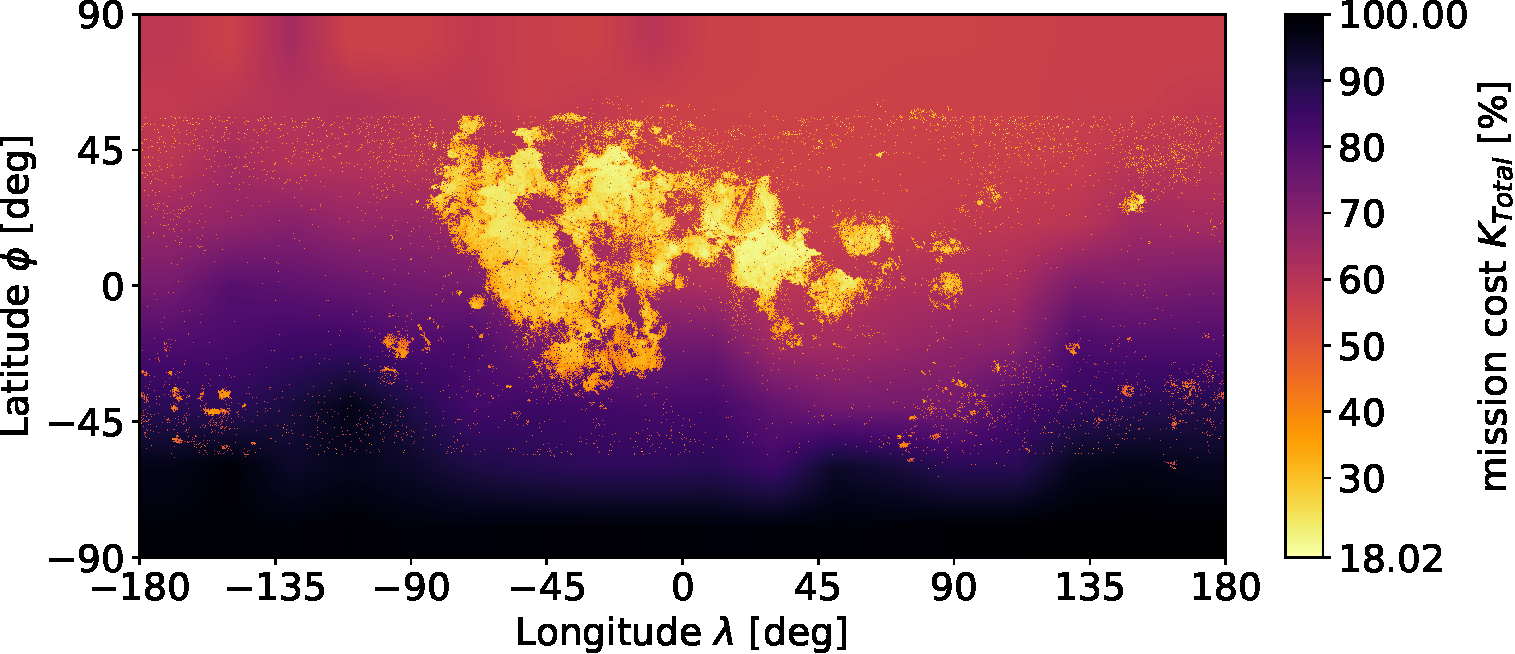
\includegraphics[width=\linewidth]{img/Total_Cost_NRHO_1_5.pdf}
\end{center}
\caption{Location dependent total mission cost $K_{\mathrm{Total}}$ in \% with $t=20$ years and $r_{\mathrm{m}}=8.6$}
\label{fig:Total_Cost_NRHO_1_5}
\end{figure}

\begin{figure}[h!]
\begin{center}
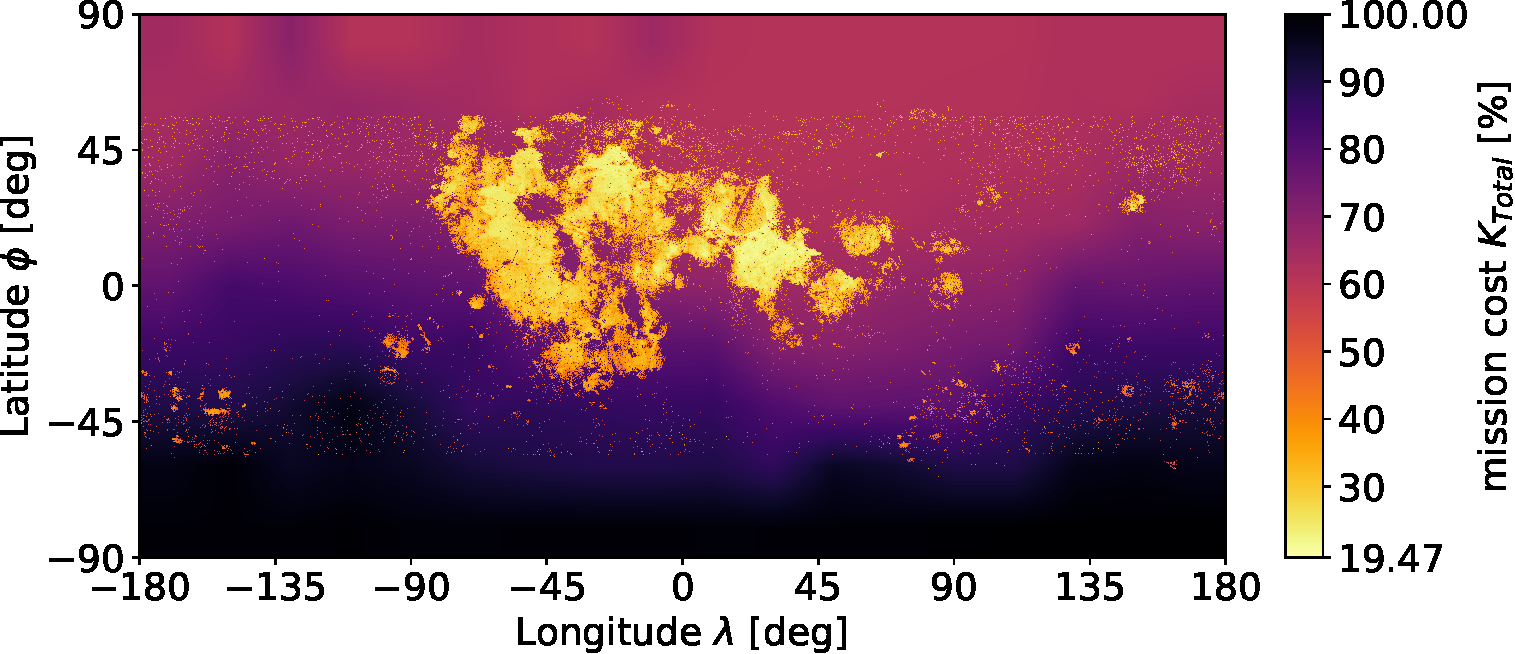
\includegraphics[width=\linewidth]{img/Total_Cost_NRHO_2_0.pdf}
\end{center}
\caption{Location dependent total mission cost $K_{\mathrm{Total}}$ in \% with $t=20$ years and $r_{\mathrm{m}}=10.7$}
\label{fig:Total_Cost_NRHO_2_0}
\end{figure}

In the direct comparison between Figure \ref{fig:Total_Cost_NRHO_1_5} and Figure \ref{fig:Total_Cost_NRHO_2_0}, the flight cost influence is visibly less pronounced for the increased mass ratio. Also, a reduced variation in total mission cost can be observed. 


\newpage
\section{Results}
\label{sec:results}

\subsection{Flight Cost Influences}

In the case of the availability of the long duration transfer (Section \ref{sec:transfer-options}) which is able to diminish location dependencies almost completely, as well as insignificant celestial influences (Section \ref{chap:planetary_influences}), the effects on the missions location selection are eliminated by an assumable uniform $\Delta v$ requirement.

Only under the short duration transfer strategy of a direct ascent, location dependent $\Delta v$ requirements are prominent (Section \ref{sec:dv-map}) which translate to a significant difference in spent fuel (Section \ref{sec:spent-fuel}). On the other side at the ISRU influence, Ilmenite reduction introduces vast location dependencies (Section \ref{sec:ISRU-map}), which overshadow the differences in the spent fuel, resulting in an ISRU feature dominated total cost when both influences are combined (Section \ref{sec:total-map}).

\subsection{Flight Cost Insignificance}

To provide insight on the induced error when the flight costs are neglected completely, the best locations from the ISRU model from Section \ref{sec:A} are compared to the best locations from the Joined model from Section \ref{sec:joined-model}.
In order to limit the possible locations, both models location dependent results are reduced into geodetic square tiles of  $15^{\circ}$, $5^{\circ}$  and $1^{\circ} (\phi , \lambda)$, to compare the behaviour on multiple resolutions.
The creation of the tiles $T_{\phi \ index, \lambda \ index}$ was performed considering pixel area relation and yields an index resolution of $12 \times 24$, $36 \times 72$ and $180 \times 360$.
From the created tiles, the top 10 choices are ranked and compared over the models. The top 10 choices make up the top 3.47 \% for the $15^{\circ}$ tiles, the top 0.39 \% for the $5^{\circ}$ tiles and the top 0.015 \% for the $1^{\circ}$ tiles.
In Table \ref{tab:location-selection-result}, the tiles are colorized by the ranking of the ISRU model, from green as most optimal to orange as less optimal locations, giving the baseline for comparison of ordering and featured tiles.
Underneath the Joined model is shown in tree time steps, at 0, 10 and 20 years, providing a sense of temporal evolution of the featured tiles. 

\begin{table}[h!]
\centering
\begin{tabular}{lllllllllll}
$15^{\circ}$ tiles & \#1                                  & \#2                                  & \#3                                  & \#4                                  & \#5                                  & \#6                                  & \#7                                  & \#8                                  & \#9                                  & \#10                                 \\
ISRU               & \cellcolor[HTML]{00FF00}$T_{5,8}$    & \cellcolor[HTML]{88FF00}$T_{5,13}$   & \cellcolor[HTML]{B8FF00}$T_{3,10}$   & \cellcolor[HTML]{E8FF00}$T_{4,7}$    & \cellcolor[HTML]{FFFF00}$T_{6,9}$    & \cellcolor[HTML]{FFEE00}$T_{3,8}$    & \cellcolor[HTML]{FFDD00}$T_{5,14}$   & \cellcolor[HTML]{FFCC00}$T_{4,13}$   & \cellcolor[HTML]{FFBB00}$T_{6,8}$    & \cellcolor[HTML]{FFAA00}$T_{4,10}$   \\
J. t = 0           & \cellcolor[HTML]{00FF00}$T_{5,8}$    & \cellcolor[HTML]{88FF00}$T_{5,13}$   & \cellcolor[HTML]{B8FF00}$T_{3,10}$   & \cellcolor[HTML]{E8FF00}$T_{4,7}$    & \cellcolor[HTML]{FFEE00}$T_{3,8}$    & \cellcolor[HTML]{FFCC00}$T_{4,13}$   & \cellcolor[HTML]{FFDD00}$T_{5,14}$   & \cellcolor[HTML]{FFFF00}$T_{6,9}$    & \cellcolor[HTML]{FFAA00}$T_{4,10}$   & $T_{5,11}$                           \\
J. t = 10          & \cellcolor[HTML]{88FF00}$T_{5,13}$   & \cellcolor[HTML]{B8FF00}$T_{3,10}$   & \cellcolor[HTML]{00FF00}$T_{5,8}$    & \cellcolor[HTML]{FFCC00}$T_{4,13}$   & \cellcolor[HTML]{E8FF00}$T_{4,7}$    & \cellcolor[HTML]{FFEE00}$T_{3,8}$    & \cellcolor[HTML]{FFDD00}$T_{5,14}$   & \cellcolor[HTML]{FFFF00}$T_{6,9}$    & \cellcolor[HTML]{FFAA00}$T_{4,10}$   & $T_{5,11}$                           \\
J. t = 20          & \cellcolor[HTML]{88FF00}$T_{5,13}$   & \cellcolor[HTML]{B8FF00}$T_{3,10}$   & \cellcolor[HTML]{00FF00}$T_{5,8}$    & \cellcolor[HTML]{FFCC00}$T_{4,13}$   & \cellcolor[HTML]{FFDD00}$T_{5,14}$   & \cellcolor[HTML]{FFEE00}$T_{3,8}$    & \cellcolor[HTML]{E8FF00}$T_{4,7}$    & \cellcolor[HTML]{FFAA00}$T_{4,10}$   & $T_{4,12}$                           & $T_{5,11}$                           \\
                   &                                      &                                      &                                      &                                      &                                      &                                      &                                      &                                      &                                      &                                      \\
$5^{\circ}$ tiles  & \#1                                  & \#2                                  & \#3                                  & \#4                                  & \#5                                  & \#6                                  & \#7                                  & \#8                                  & \#9                                  & \#10                                 \\
ISRU               & \cellcolor[HTML]{00FF00}$T_{15,40}$  & \cellcolor[HTML]{88FF00}$T_{14,24}$  & \cellcolor[HTML]{B8FF00}$T_{16,41}$  & \cellcolor[HTML]{E8FF00}$T_{14,23}$  & \cellcolor[HTML]{FFFF00}$T_{16,40}$  & \cellcolor[HTML]{FFEE00}$T_{12,23}$  & \cellcolor[HTML]{FFDD00}$T_{10,31}$  & \cellcolor[HTML]{FFCC00}$T_{13,24}$  & \cellcolor[HTML]{FFBB00}$T_{15,25}$  & \cellcolor[HTML]{FFAA00}$T_{15,42}$  \\
J. t = 0           & \cellcolor[HTML]{00FF00}$T_{15,40}$  & \cellcolor[HTML]{B8FF00}$T_{16,41}$  & \cellcolor[HTML]{FFFF00}$T_{16,40}$  & \cellcolor[HTML]{88FF00}$T_{14,24}$  & \cellcolor[HTML]{FFDD00}$T_{10,31}$  & \cellcolor[HTML]{FFAA00}$T_{15,42}$  & $T_{15,43}$                          & \cellcolor[HTML]{E8FF00}$T_{14,23}$  & $T_{15,41}$                          & $T_{16,42}$                          \\
J. t = 10          & \cellcolor[HTML]{00FF00}$T_{15,40}$  & \cellcolor[HTML]{B8FF00}$T_{16,41}$  & \cellcolor[HTML]{FFFF00}$T_{16,40}$  & \cellcolor[HTML]{FFAA00}$T_{15,42}$  & \cellcolor[HTML]{FFDD00}$T_{10,31}$  & $T_{15,43}$                          & $T_{15,41}$                          & $T_{16,42}$                          & $T_{17,40}$                          & $T_{11,31}$                          \\
J. t = 20          & \cellcolor[HTML]{00FF00}$T_{15,40}$  & \cellcolor[HTML]{B8FF00}$T_{16,41}$  & \cellcolor[HTML]{FFAA00}$T_{15,42}$  & $T_{15,43}$                          & \cellcolor[HTML]{FFFF00}$T_{16,40}$  & \cellcolor[HTML]{FFDD00}$T_{10,31}$  & $T_{15,41}$                          & $T_{16,42}$                          & $T_{11,31}$                          & $T_{14,41}$                          \\
                   &                                      &                                      &                                      &                                      &                                      &                                      &                                      &                                      &                                      &                                      \\
$1^{\circ}$ tiles  & \#1                                  & \#2                                  & \#3                                  & \#4                                  & \#5                                  & \#6                                  & \#7                                  & \#8                                  & \#9                                  & \#10                                 \\
ISRU               & \cellcolor[HTML]{00FF00}$T_{79,204}$ & \cellcolor[HTML]{88FF00}$T_{81,201}$ & \cellcolor[HTML]{B8FF00}$T_{80,200}$ & \cellcolor[HTML]{E8FF00}$T_{72,118}$ & \cellcolor[HTML]{FFFF00}$T_{80,201}$ & \cellcolor[HTML]{FFEE00}$T_{84,171}$ & \cellcolor[HTML]{FFDD00}$T_{72,117}$ & \cellcolor[HTML]{FFCC00}$T_{81,199}$ & \cellcolor[HTML]{FFBB00}$T_{72,116}$ & \cellcolor[HTML]{FFAA00}$T_{80,204}$ \\
J. t = 0           & \cellcolor[HTML]{00FF00}$T_{79,204}$ & \cellcolor[HTML]{88FF00}$T_{81,201}$ & \cellcolor[HTML]{B8FF00}$T_{80,200}$ & \cellcolor[HTML]{FFFF00}$T_{80,201}$ & \cellcolor[HTML]{FFAA00}$T_{80,204}$ & \cellcolor[HTML]{FFCC00}$T_{81,199}$ & $T_{80,203}$                         & $T_{79,203}$                         & $T_{80,199}$                         & $T_{81,200}$                         \\
J. t = 10          & \cellcolor[HTML]{00FF00}$T_{79,204}$ & \cellcolor[HTML]{B8FF00}$T_{80,200}$ & \cellcolor[HTML]{FFFF00}$T_{80,201}$ & $T_{81,201}$                         & \cellcolor[HTML]{FFAA00}$T_{80,204}$ & $T_{79,203}$                         & $T_{80,203}$                         & $T_{76,201}$                         & $T_{78,218}$                         & $T_{78,204}$                         \\
J. t = 20          & \cellcolor[HTML]{00FF00}$T_{79,204}$ & $T_{71,206}$                         & $T_{78,218}$                         & $T_{76,201}$                         & $T_{75,206}$                         & $T_{77,212}$                         & $T_{76,206}$                         & \cellcolor[HTML]{FFAA00}$T_{80,204}$ & \cellcolor[HTML]{FFFF00}$T_{80,201}$ & $T_{79,203}$                        
\end{tabular}
\caption{Top 10 best mission locations compared between ISRU model and Joined model (J.) after t years in pixel area relation resized square tiles ($T_{\phi \ index, \lambda \ index}$) with resolution $\phi , \lambda$ of $15^{\circ}$ (top) $,5^{\circ}$ (middle) and $1^{\circ}$ (bottom). Indices starting at zero on $(90^{\circ} \phi, -180^{\circ} \lambda)$ with $-180^{\circ}$ to $180^{\circ}$ Longitude range. Data from mass ratio $r_{\mathrm{m}}=8.6$.}
\label{tab:location-selection-result}
\end{table}

The induced error of the flight cost neglect increases over mission time, but nevertheless even at greater time spans as 20 years, the top 10 of the Joined model are featuring many tiles which have been in the top 10 of the ISRU ranking.
The increased conservation of the highest ranked tiles can be explained by the coincidental overlap of low flight costs and low ISRU costs.
In higher resolutions less tiles are shared, however due to the difference in percentage the top 10 make up for the whole set, the shared tiles are remaining substantial.
Therefore, from Table \ref{tab:location-selection-result} is concluded that the induced error during location selection is found to be small enough that a simplification, to only consider the ISRU effects, appears a valid approximation even for greater differences in $\Delta v$ as in the analysed case.


\section{Discussion}
\label{sec:Discussion}

The identification of the secondary relevance and even neglect of flight costs in the selected mission scenario can not directly be generalized without requirements, as for other ISRU production methods, target orbits, trajectories or mass ratios each of their influence can differ greatly from the analysed case.

However, under the given case of Ilmenite reduction and transport properties that are comparable or weaker than the analysed case, flight costs differences can be assumed insignificant.
In particular, the major influence to verify in a quick assessment of a general case is the estimation of differences in $\Delta v$ requirements, which should be less than the analysed case of $\approx 20 \%$. Lower mass ratios of the launcher are amplifying these differences in $\Delta v$ when transferred to spent fuel and therefore fuel costs. 
Furthermore should be mentioned that this analysis featured a scenario which involved propellant refilling by own entities which reduces the fuel costs in general, which needs to be considered when other cost modelling is present.
Additionally, the flight frequency is scaling up flight costs linearly and can compress the shift over time for the most optimal location, where as a rough reference value the delivered payload of $8 \ t$ per year can be considered from the analysed case.

Although a significant difference in the accessibility of the southern hemisphere was the result of the direct ascent trajectory, it needs to be underlined that this does not conclude a worse accessibility from the NRHO to the southern hemisphere in general. In the chosen set of trajectories no options for intermediate parking orbits are considered, which however if considered would bring these differences between northern and southern hemisphere down, as the 1 day transfer in \cite{May2020} shows entirely different characteristics.

As global lunar data is increasingly present, problems as these can be analysed and optimised close to their entirety over the whole lunar surface.
Especially in the current stage of time where no infrastructure is yet deployed on the lunar surface, location selection can be carried by optimisation instead of dependencies by prior infrastructure.

To not create a prior infrastructure restriction ourselves, the plan for man-kinds presence and economics and even sustainability on the Moon should be expanded and seen in a bigger scope as much as possible. As this Oxygen propellant facility is just one entity of an economics network, which might move its most optimal location completely away in bigger context from its individually analysed location. Such a large scale technical investigation would make for a compelling future study.

\section*{Conflict of Interest Statement}
The authors declare hereby that the research was conducted in the absence of any commercial or financial relationships that could be construed as a potential conflict of interest.

\section*{Author Contributions}
SS conducted the research, created the solution methods and wrote the paper.
PZ did initiate the papers idea, supervised the research and reviewed the manuscript.
DQ discussed orbital mechanics aspects and reviewed the manuscript. 

\section*{Funding}
This research was conducted without any institutional funding.
Publication fees are covered by the publication fund of the German Aerospace Center (DLR) in support for open access publishing.

\section*{Data Availability Statement}
This work is providing open source on all processing steps performed in the corresponding Python Notebooks along with all resources in full resolution in the papers \href{https://redirect.sven-j-steinert.de/?id=2023_DLR}{\underline{Git-Repository}}.

% Please see the availability of data guidelines for more information, at https://www.frontiersin.org/guidelines/policies-and-publication-ethics#materials-and-data-policies

\bibliographystyle{Frontiers-Harvard} %  Many Frontiers journals use the Harvard referencing system (Author-date), to find the style and resources for the journal you are submitting to: https://zendesk.frontiersin.org/hc/en-us/articles/360017860337-Frontiers-Reference-Styles-by-Journal. For Humanities and Social Sciences articles please include page numbers in the in-text citations 
%\bibliographystyle{Frontiers-Vancouver} % Many Frontiers journals use the numbered referencing system, to find the style and resources for the journal you are submitting to: https://zendesk.frontiersin.org/hc/en-us/articles/360017860337-Frontiers-Reference-Styles-by-Journal

\bibliography{bibliography}

%%% Make sure to upload the bib file along with the tex file and PDF
%%% Please see the test.bib file for some examples of references

%\section*{Figure captions}

%%% Please be aware that for original research articles we only permit a combined number of 15 figures and tables, one figure with multiple subfigures will count as only one figure.
%%% Use this if adding the figures directly in the mansucript, if so, please remember to also upload the files when submitting your article
%%% There is no need for adding the file termination, as long as you indicate where the file is saved. In the examples below the files (logo1.eps and logos.eps) are in the Frontiers LaTeX folder
%%% If using *.tif files convert them to .jpg or .png
%%%  NB logo1.eps is required in the path in order to correctly compile front page header %%%


%%% If you don't add the figures in the LaTeX files, please upload them when submitting the article.
%%% Frontiers will add the figures at the end of the provisional pdf automatically
%%% The use of LaTeX coding to draw Diagrams/Figures/Structures should be avoided. They should be external callouts including graphics.

\end{document}
